\documentclass[a4paper,12pt]{article}
\usepackage[margin=2cm]{geometry}
\usepackage{tikz}
\usetikzlibrary{shapes.geometric, arrows.meta, positioning, fit, backgrounds}
\usepackage{booktabs}
\usepackage{tabularx}
\usepackage{array}
\usepackage{xcolor}
\usepackage{caption}
\usepackage{lmodern}
\usepackage{colortbl}

% ── Colour palette ─────────────────────────────────────────────
\definecolor{stage1bg}{RGB}{220,235,252}   % soft blue
\definecolor{stage1bd}{RGB}{52,109,193}
\definecolor{stage2bg}{RGB}{255,243,205}   % soft amber
\definecolor{stage2bd}{RGB}{214,158,46}
\definecolor{stage3bg}{RGB}{212,237,218}   % soft green
\definecolor{stage3bd}{RGB}{40,140,80}
\definecolor{arrowcol}{RGB}{90,90,90}
\definecolor{headerbg}{RGB}{44,62,100}     % dark navy
\definecolor{rowodd}{RGB}{245,248,255}
\definecolor{roweven}{RGB}{255,255,255}

\begin{document}

% ══════════════════════════════════════════════════════════════════
%  FIGURE 3.1 – Planning Evolution Framework
% ══════════════════════════════════════════════════════════════════
\section*{Figure 3.1: Evolution of the IAMS Project Planning Strategy}

\begin{figure}[h]
\centering
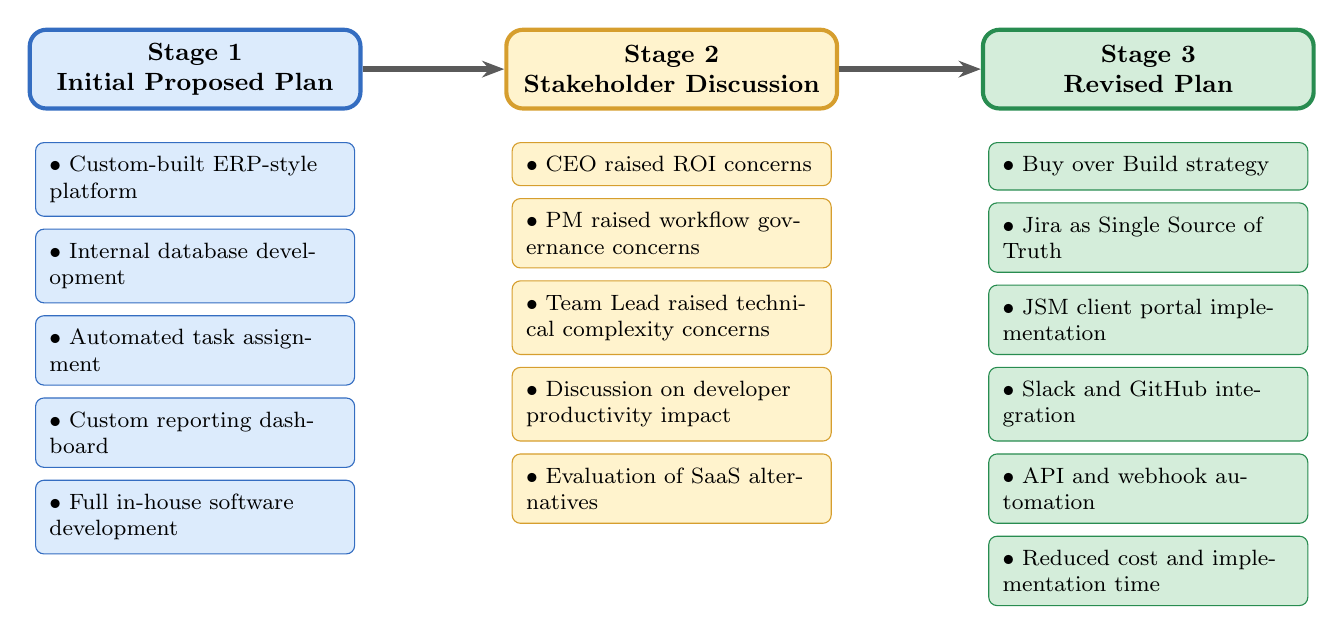
\begin{tikzpicture}[
    node distance = 1.6cm,
    box/.style    = {rectangle, rounded corners=6pt, minimum width=4.2cm,
                     minimum height=1cm, align=center, font=\bfseries\small},
    item/.style   = {rectangle, rounded corners=3pt, minimum width=3.9cm,
                     text width=3.7cm, align=left, font=\footnotesize,
                     inner sep=5pt},
    arrow/.style  = {-{Stealth[length=8pt,width=6pt]}, line width=2pt,
                     color=arrowcol},
]

% ── Stage headers ───────────────────────────────────────────────
\node[box, fill=stage1bg, draw=stage1bd, line width=1.5pt] (h1)
    {Stage 1\\Initial Proposed Plan};

\node[box, fill=stage2bg, draw=stage2bd, line width=1.5pt,
      right=1.8cm of h1] (h2)
    {Stage 2\\Stakeholder Discussion};

\node[box, fill=stage3bg, draw=stage3bd, line width=1.5pt,
      right=1.8cm of h2] (h3)
    {Stage 3\\Revised Plan};

% ── Arrows between headers ──────────────────────────────────────
\draw[arrow] (h1.east) -- (h2.west);
\draw[arrow] (h2.east) -- (h3.west);

% ── Stage 1 bullet items ────────────────────────────────────────
\node[item, fill=stage1bg, draw=stage1bd, below=0.4cm of h1] (i1a)
    {$\bullet$\ Custom-built ERP-style platform};
\node[item, fill=stage1bg, draw=stage1bd, below=0.15cm of i1a] (i1b)
    {$\bullet$\ Internal database development};
\node[item, fill=stage1bg, draw=stage1bd, below=0.15cm of i1b] (i1c)
    {$\bullet$\ Automated task assignment};
\node[item, fill=stage1bg, draw=stage1bd, below=0.15cm of i1c] (i1d)
    {$\bullet$\ Custom reporting dashboard};
\node[item, fill=stage1bg, draw=stage1bd, below=0.15cm of i1d] (i1e)
    {$\bullet$\ Full in-house software development};

% ── Stage 2 bullet items ────────────────────────────────────────
\node[item, fill=stage2bg, draw=stage2bd, below=0.4cm of h2] (i2a)
    {$\bullet$\ CEO raised ROI concerns};
\node[item, fill=stage2bg, draw=stage2bd, below=0.15cm of i2a] (i2b)
    {$\bullet$\ PM raised workflow governance concerns};
\node[item, fill=stage2bg, draw=stage2bd, below=0.15cm of i2b] (i2c)
    {$\bullet$\ Team Lead raised technical complexity concerns};
\node[item, fill=stage2bg, draw=stage2bd, below=0.15cm of i2c] (i2d)
    {$\bullet$\ Discussion on developer productivity impact};
\node[item, fill=stage2bg, draw=stage2bd, below=0.15cm of i2d] (i2e)
    {$\bullet$\ Evaluation of SaaS alternatives};

% ── Stage 3 bullet items ────────────────────────────────────────
\node[item, fill=stage3bg, draw=stage3bd, below=0.4cm of h3] (i3a)
    {$\bullet$\ Buy over Build strategy};
\node[item, fill=stage3bg, draw=stage3bd, below=0.15cm of i3a] (i3b)
    {$\bullet$\ Jira as Single Source of Truth};
\node[item, fill=stage3bg, draw=stage3bd, below=0.15cm of i3b] (i3c)
    {$\bullet$\ JSM client portal implementation};
\node[item, fill=stage3bg, draw=stage3bd, below=0.15cm of i3c] (i3d)
    {$\bullet$\ Slack and GitHub integration};
\node[item, fill=stage3bg, draw=stage3bd, below=0.15cm of i3d] (i3e)
    {$\bullet$\ API and webhook automation};
\node[item, fill=stage3bg, draw=stage3bd, below=0.15cm of i3e] (i3f)
    {$\bullet$\ Reduced cost and implementation time};

\end{tikzpicture}

\caption{Evolution of the IAMS project planning strategy from an initial custom
software proposal to a SaaS-based integration architecture following stakeholder
review.}
\end{figure}

\clearpage

% ══════════════════════════════════════════════════════════════════
%  TABLE 3.1 – Comparison of Initial and Revised Plan
% ══════════════════════════════════════════════════════════════════
\section*{Table 3.1: Comparison of Initial Proposed Plan and Revised Integration Plan}

\begin{table}[h]
\centering
\renewcommand{\arraystretch}{1.45}
\small
\begin{tabularx}{\textwidth}{
    >{\bfseries}p{4.2cm}          % Planning Area
    >{\raggedright\arraybackslash}X  % Initial Plan
    >{\raggedright\arraybackslash}X  % Revised Plan
}
\toprule
\rowcolor{headerbg}
\textcolor{white}{\textbf{Planning Area}} &
\textcolor{white}{\textbf{Initial Proposed Plan}} &
\textcolor{white}{\textbf{Revised Integration Plan}} \\
\midrule

\rowcolor{rowodd}
Development Approach &
Custom-built internal platform &
SaaS integration architecture \\

\rowcolor{roweven}
Core Technology &
Custom database and application &
Jira, JSM, Slack, GitHub, ScriptRunner \\

\rowcolor{rowodd}
Project Duration &
Estimated 6–12 months &
12-week deployment \\

\rowcolor{roweven}
Development Effort &
Full-scale software development &
Configuration and integration \\

\rowcolor{rowodd}
Cost Structure &
High variable development cost &
Predictable SaaS licensing cost \\

\rowcolor{roweven}
Developer Resource Usage &
Heavy internal resource consumption &
Minimal disruption to billable work \\

\rowcolor{rowodd}
Workflow Management &
Custom workflow implementation &
Jira-based workflow automation \\

\rowcolor{roweven}
Client Communication &
Direct system interaction &
Structured JSM portal \\

\rowcolor{rowodd}
Maintenance Responsibility &
Fully internal maintenance &
Vendor-supported SaaS ecosystem \\

\rowcolor{roweven}
ROI Outlook &
Delayed and uncertain &
Faster and more predictable \\

\bottomrule
\end{tabularx}

\caption{Comparative analysis between the original custom development proposal
and the revised SaaS-based integration strategy adopted for the IAMS project.}
\end{table}

\end{document}